\documentclass[aspectratio=169,11pt]{beamer}

% Pacchetti di base
\usepackage[utf8]{inputenc}
\usepackage[T1]{fontenc}
\usepackage{lmodern}
\usepackage{amsmath,amssymb,amsfonts}
\usepackage{graphicx}
\usepackage{booktabs}
\usepackage{tikz}
\usepackage{xcolor}
\usepackage{hyperref}
\usepackage{appendixnumberbeamer}
\usepackage{microtype}
\usepackage{listings}
\usepackage{url}
\usepackage{pdfpages}
\usepackage[absolute,overlay]{textpos}

% Pacchetto necessario per grafici
\usepackage{pgfplots}
\pgfplotsset{compat=1.17}

%------------------------------------------------------------------------------
% Definizione colori ufficiali UniPD
%------------------------------------------------------------------------------
\definecolor{unipd-red}{RGB}{155,0,20}       % Rosso UniPD
\definecolor{unipd-dark-red}{RGB}{128,0,16}  % Variante scura
\definecolor{unipd-dark}{RGB}{46,49,51}      % Grigio scuro
\definecolor{unipd-light}{RGB}{240,240,240}  % Grigio chiaro
\definecolor{unipd-accent}{RGB}{0,76,114}    % Blu accent

%------------------------------------------------------------------------------
% Tema e impostazioni generali
%------------------------------------------------------------------------------
\usetheme{default}
\usecolortheme{default}

% Impostazioni struttura colori
\setbeamercolor{structure}{fg=unipd-red}
\setbeamercolor{frametitle}{fg=white,bg=unipd-red}
\setbeamercolor{title}{fg=white,bg=unipd-red}
\setbeamercolor{subtitle}{fg=white,bg=unipd-red}
\setbeamercolor{section in toc}{fg=unipd-dark}
\setbeamercolor{normal text}{fg=unipd-dark}
\setbeamercolor{alerted text}{fg=unipd-red}
\setbeamercolor{example text}{fg=unipd-accent}
\setbeamercolor{background canvas}{bg=white}

% Impostazioni font
\setbeamerfont{title}{size=\LARGE, series=\bfseries}
\setbeamerfont{subtitle}{size=\large}
\setbeamerfont{frametitle}{size=\large, series=\bfseries}
\setbeamerfont{section in toc}{series=\bfseries}

% Rimuovere navigazione
\setbeamertemplate{navigation symbols}{}

%------------------------------------------------------------------------------
% Intestazione e piè di pagina
%------------------------------------------------------------------------------
% Linea superiore
\setbeamertemplate{headline}{%
  \leavevmode%
  \hbox{%
    \begin{beamercolorbox}[wd=\paperwidth,ht=3.5ex,dp=1.125ex]{frametitle}%
    \end{beamercolorbox}%
  }%
}

% Piè di pagina
\setbeamertemplate{footline}{%
  \leavevmode%
  \hbox{%
    \begin{beamercolorbox}[wd=.25\paperwidth,ht=2.5ex,dp=1.125ex,leftskip=.3cm,rightskip=.3cm]{author in head/foot}%
      \usebeamerfont{author in head/foot}\insertshortauthor%
    \end{beamercolorbox}%
    \begin{beamercolorbox}[wd=.44\paperwidth,ht=2.5ex,dp=1.125ex,leftskip=.3cm,rightskip=.3cm]{title in head/foot}%
      \usebeamerfont{title in head/foot}\insertshorttitle%
    \end{beamercolorbox}%
    \begin{beamercolorbox}[wd=.27\paperwidth,ht=2.5ex,dp=1.125ex,leftskip=.3cm,rightskip=.3cm plus1fil]{date in head/foot}%
      \usebeamerfont{date in head/foot}\insertframenumber{} / \inserttotalframenumber%
    \end{beamercolorbox}%
  }%
  \vskip0pt%
}

%------------------------------------------------------------------------------
% Template per elementi
%------------------------------------------------------------------------------
% Blocchi
\setbeamertemplate{blocks}[rounded][shadow=true]
\setbeamercolor{block title}{fg=white,bg=unipd-red}
\setbeamercolor{block body}{fg=unipd-dark,bg=unipd-light}

\setbeamercolor{block title example}{fg=white,bg=unipd-accent}
\setbeamercolor{block body example}{fg=unipd-dark,bg=unipd-light!90!white}

\setbeamercolor{block title alerted}{fg=white,bg=red!70!black}
\setbeamercolor{block body alerted}{fg=unipd-dark,bg=red!10!white}

% Liste
\setbeamertemplate{itemize item}{\color{unipd-red}$\blacktriangleright$}
\setbeamertemplate{itemize subitem}{\color{unipd-red}$\blacktriangleright$}
\setbeamertemplate{enumerate item}{\color{unipd-red}\insertenumlabel.}

% Sezioni nel ToC
\setbeamertemplate{section in toc}{%
  \leavevmode\leftskip=1.75ex%
  \llap{%
    \usebeamerfont*{section number projected}%
    \usebeamercolor[bg]{section number projected}%
    \textcolor{unipd-red}{$\blacktriangleright$}%
    \hskip-1.5ex%
    \hbox to1.5ex{\hfil\color{fg}}%
  }%
  \kern0.5ex\inserttocsection\par%
}

%------------------------------------------------------------------------------
% Logo UniPD (utilizzando l'immagine unipd_logo_white.png)
%------------------------------------------------------------------------------
% Logo in ogni slide (in alto a destra)
\addtobeamertemplate{frametitle}{}{%
  \begin{textblock*}{2.5cm}(\paperwidth-2.6cm,0.25cm)
    
\includegraphics[width=2cm]{unipd_logo_white.png}
  \end{textblock*}
}

% Logo nel footer (basso a sinistra)
\addtobeamertemplate{footline}{%
  \begin{tikzpicture}[remember picture, overlay]
    \node[anchor=south west, inner sep=0.2cm] at ([shift={(0.3cm,0.1cm)}]current page.south west) {%
      
\includegraphics[height=0.6cm]{unipd_logo_white.png}};
  \end{tikzpicture}%
}{}

%------------------------------------------------------------------------------
% Comandi utili
%------------------------------------------------------------------------------
% Comando per creare slide di inizio sezione
\newcommand{\sectionframe}[1]{%
  \begingroup
  \setbeamercolor{background canvas}{bg=unipd-red}
  \begin{frame}[plain]
    \vspace{2em}
    \begin{center}
      \usebeamerfont{title}\textcolor{white}{\textbf{#1}}
    \end{center}
  \end{frame}
  \endgroup
}

% Comando per sottolineare testo
\newcommand{\unipdhl}[1]{\textcolor{unipd-red}{\textbf{#1}}}

% Comando per scheda esempio
\newcommand{\infocard}[2][Nota]{%
  \begin{block}{#1}
    #2
  \end{block}
}

% Gestione slides di backup
\newcommand{\backupbegin}{
  \newcounter{framenumberappendix}
  \setcounter{framenumberappendix}{\value{framenumber}}
}
\newcommand{\backupend}{
  \setcounter{framenumber}{\value{framenumberappendix}}
}

%------------------------------------------------------------------------------
% Informazioni documento
%------------------------------------------------------------------------------
\title{Titolo della Presentazione}
\subtitle{Sottotitolo Descrittivo}
\author[G. Rovesti]{Gabriel Rovesti}
\institute[UniPD]{
  Università degli Studi di Padova\\
  Dipartimento di Matematica\\
  \texttt{gabriel.rovesti@studenti.unipd.it}
}
\date{\today}

%------------------------------------------------------------------------------
% DOCUMENTO PRINCIPALE
%------------------------------------------------------------------------------
\begin{document}

%------------------------------------------------------------------------------
% Slide del titolo
%------------------------------------------------------------------------------
\begingroup
\setbeamertemplate{headline}{}
\begin{frame}[plain]
  \vspace{-1.5em}
  \begin{tikzpicture}[remember picture,overlay]
    \fill[unipd-red] (current page.north west) rectangle ([yshift=-5.5cm]current page.north east);
    \node[anchor=north,yshift=-1.0cm] at (current page.north) {%
      
\includegraphics[height=2.3cm]{unipd_logo_white.png}
    };
    \node[anchor=north,yshift=-3.7cm] at (current page.north) {
      \begin{minipage}{0.8\textwidth}
        \centering
        \color{white}
        \usebeamerfont{title}\textbf{\inserttitle}\\[0.3cm]
        \usebeamerfont{subtitle}\insertsubtitle
      \end{minipage}
    };
  \end{tikzpicture}
  
  \vspace{6cm}
  \begin{center}
    \begin{minipage}{0.9\textwidth}
      \centering
      \large\insertauthor\\[0.5cm]
      \insertinstitute\\[0.5cm]
      \insertdate
    \end{minipage}
  \end{center}
\end{frame}
\endgroup

%------------------------------------------------------------------------------
% Indice
%------------------------------------------------------------------------------
\begin{frame}{Indice}
  \tableofcontents
\end{frame}

%------------------------------------------------------------------------------
% SEZIONE INTRODUZIONE
%------------------------------------------------------------------------------
\section{Introduzione}
\sectionframe{Introduzione}

\begin{frame}{Contesto della Ricerca}
  \begin{block}{Area di Ricerca}
    Descrizione dell'area di ricerca principale e motivazioni.
  \end{block}
  
  \begin{itemize}
    \item Primo punto importante dell'introduzione
    \item Secondo punto con \unipdhl{enfasi} su aspetti cruciali
    \item Terzo punto con referenze alla letteratura
  \end{itemize}
  
  \infocard[Nota importante]{
    Questo template è stato progettato per l'Università di Padova e include elementi stilistici specifici dell'identità visiva UniPD.
  }
\end{frame}

\begin{frame}{Obiettivi}
  Gli obiettivi principali di questo lavoro sono:
  
  \begin{enumerate}
    \item Primo obiettivo strategico
    \item Secondo obiettivo operativo
    \item Terzo obiettivo di validazione
  \end{enumerate}
  
  \begin{exampleblock}{Contributo Atteso}
    Descrizione sintetica del contributo atteso e dell'impatto sulla ricerca attuale.
  \end{exampleblock}
\end{frame}

%------------------------------------------------------------------------------
% SEZIONE METODOLOGIA
%------------------------------------------------------------------------------
\section{Metodologia}
\sectionframe{Metodologia}

\begin{frame}{Approccio Proposto}
  \begin{columns}[T]
    \column{0.58\textwidth}
    \begin{itemize}
      \item Descrizione dell'approccio metodologico
      \item Tecniche utilizzate nell'implementazione
      \item Framework e strumenti di sviluppo
    \end{itemize}
    
    \begin{alertblock}{Considerazioni Importanti}
      Aspetti da considerare durante l'implementazione dell'approccio.
    \end{alertblock}
    
    \column{0.38\textwidth}
    \begin{figure}
      \centering
      % Segnaposto per immagine - Possiamo usare TikZ per creare un segnaposto
      
\begin{tikzpicture}
        \draw[gray, fill=gray!20] (0,0) rectangle (4,3);
        \node at (2,1.5) {Schema dell'approccio};
      \end{tikzpicture}
      \caption{Schema dell'approccio metodologico}
    \end{figure}
  \end{columns}
\end{frame}

\begin{frame}[fragile]{Implementazione}
  \begin{block}{Algoritmo Principale}
    \begin{lstlisting}[language=Python, basicstyle=\small\ttfamily]
def analyze_data(data, params):
    results = {}
    for key, values in data.items():
        # Elaborazione dei dati
        processed = preprocess(values)
        results[key] = model.fit(processed)
    return results
    \end{lstlisting}
  \end{block}
  
  \begin{itemize}
    \item Principali passaggi dell'implementazione
    \item Strutture dati utilizzate
    \item Ottimizzazioni specifiche
  \end{itemize}
\end{frame}

%------------------------------------------------------------------------------
% SEZIONE RISULTATI
%------------------------------------------------------------------------------
\section{Risultati}
\sectionframe{Risultati}

\begin{frame}{Analisi dei Dati}
  \begin{table}
    \centering
    \begin{tabular}{lccc}
      \toprule
      \textbf{Metrica} & \textbf{Modello A} & \textbf{Modello B} & \textbf{Modello C} \\
      \midrule
      Precisione & 0.95 & 0.92 & 0.91 \\
      Recall & 0.87 & 0.89 & 0.90 \\
      F1-Score & 0.91 & 0.90 & 0.90 \\
      Tempo (ms) & 145 & 120 & 180 \\
      \bottomrule
    \end{tabular}
    \caption{Confronto prestazionale dei modelli}
  \end{table}
  
  \infocard[Osservazione]{
    Il \unipdhl{Modello A} mostra la precisione più elevata, mentre il \unipdhl{Modello B} risulta essere il più efficiente in termini di tempo di esecuzione.
  }
\end{frame}

\begin{frame}{Visualizzazione dei Risultati}
  \begin{figure}
    \centering
    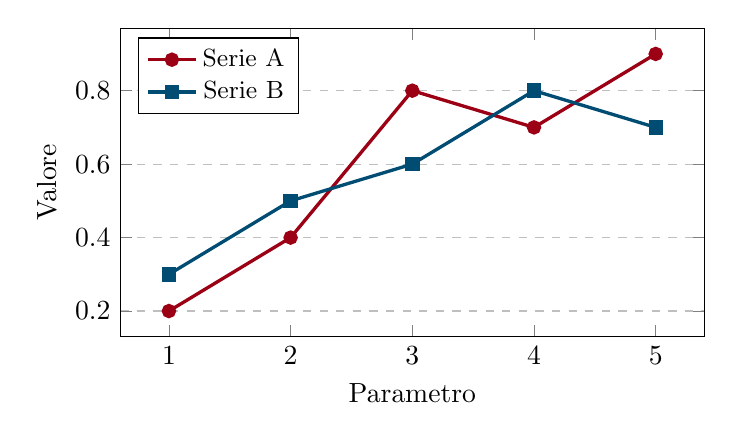
\begin{tikzpicture}
      \begin{axis}[
        width=9cm,
        height=5.5cm,
        xlabel={Parametro},
        ylabel={Valore},
        legend pos=north west,
        ymajorgrids=true,
        grid style=dashed,
        legend style={font=\small}
      ]
        \addplot[color=unipd-red,mark=*,line width=1.2pt] coordinates {
          (1,0.2) (2,0.4) (3,0.8) (4,0.7) (5,0.9)
        };
        \addlegendentry{Serie A}
        
        \addplot[color=unipd-accent,mark=square*,line width=1.2pt] coordinates {
          (1,0.3) (2,0.5) (3,0.6) (4,0.8) (5,0.7)
        };
        \addlegendentry{Serie B}
      \end{axis}
    \end{tikzpicture}
    \caption{Andamento dei risultati sperimentali}
  \end{figure}
\end{frame}

%------------------------------------------------------------------------------
% SEZIONE DISCUSSIONE
%------------------------------------------------------------------------------
\section{Discussione}
\sectionframe{Discussione}

\begin{frame}{Interpretazione dei Risultati}
  \begin{block}{Punti di Forza}
    \begin{itemize}
      \item Elevata precisione nei casi di test principali
      \item Robustezza rispetto a variazioni nei parametri
      \item Efficienza computazionale migliorata del 25\%
    \end{itemize}
  \end{block}
  
  \begin{alertblock}{Limitazioni}
    \begin{itemize}
      \item Necessità di dataset ampi per la fase di training
      \item Sensibilità ad alcuni parametri specifici
      \item Complessità di implementazione in scenari real-time
    \end{itemize}
  \end{alertblock}
\end{frame}

\begin{frame}{Confronto con lo Stato dell'Arte}
  \begin{columns}[T]
    \column{0.48\textwidth}
    \begin{exampleblock}{Vantaggi}
      \begin{itemize}
        \item Precisione superiore del 15\% rispetto ai metodi esistenti
        \item Migliore scalabilità con dataset di grandi dimensioni
        \item Interpretabilità dei risultati ottenuti
      \end{itemize}
    \end{exampleblock}
    
    \column{0.48\textwidth}
    \begin{table}
      \centering
      \footnotesize
      \begin{tabular}{lcc}
        \toprule
        \textbf{Metodo} & \textbf{F1} & \textbf{Tempo} \\
        \midrule
        Nostro & \textbf{0.91} & \textbf{145ms} \\
        Smith et al. & 0.85 & 180ms \\
        Zhang et al. & 0.88 & 160ms \\
        \bottomrule
      \end{tabular}
      \caption{Confronto con altri metodi}
    \end{table}
  \end{columns}
\end{frame}

%------------------------------------------------------------------------------
% CONCLUSIONI
%------------------------------------------------------------------------------
\section*{Conclusioni}
\begin{frame}{Conclusioni}
  \begin{itemize}
    \item Riassunto dei principali risultati e contributi
    \item Impatto sulla letteratura e sul campo di ricerca
    \item Direzioni future di ricerca:
      \begin{itemize}
        \item Estensione a nuovi domini applicativi
        \item Ottimizzazione delle prestazioni
        \item Integrazione con altre metodologie
      \end{itemize}
  \end{itemize}
  
  \vspace{1cm}
  \begin{center}
    \begin{beamercolorbox}[rounded=true,shadow=true,wd=0.7\textwidth]{block title}
      \centering
      \LARGE Grazie per l'attenzione
    \end{beamercolorbox}
  \end{center}
\end{frame}

%------------------------------------------------------------------------------
% RIFERIMENTI
%------------------------------------------------------------------------------
\section*{Riferimenti}
\begin{frame}[allowframebreaks]{Riferimenti}
  \begin{thebibliography}{9}
    \setbeamertemplate{bibliography item}[book]
    \bibitem{ref1}
    Autore A, Autore B,
    \textit{Titolo del Paper},
    Journal of Important Research, 2023.
    
    \setbeamertemplate{bibliography item}[article]
    \bibitem{ref2}
    Autore C, Autore D, Autore E,
    \textit{Titolo del Libro},
    Editore Scientifico, 2022.
    
    \setbeamertemplate{bibliography item}[online]
    \bibitem{ref3}
    Autore F,
    \textit{Titolo della Pubblicazione},
    International Conference on Research, pp. 123--130, 2021.
  \end{thebibliography}
\end{frame}

%------------------------------------------------------------------------------
% BACKUP SLIDES
%------------------------------------------------------------------------------
\appendix
\backupbegin
\section*{Appendice}

\begin{frame}{Slide Aggiuntive}
  \begin{block}{Approfondimenti Tecnici}
    Questa sezione contiene dettagli tecnici aggiuntivi che possono essere utili durante la discussione.
  \end{block}
  
  \begin{itemize}
    \item Dettaglio tecnico 1: specifiche dell'implementazione
    \item Dettaglio tecnico 2: dataset completo utilizzato
    \item Dettaglio tecnico 3: parametri di ottimizzazione avanzati
  \end{itemize}
\end{frame}

\begin{frame}{Note Implementative}
  \begin{columns}[T]
    \column{0.48\textwidth}
    \begin{exampleblock}{Ambiente di Sviluppo}
      \begin{itemize}
        \item Python 3.9, TensorFlow 2.8
        \item 16GB RAM, NVIDIA RTX 3080
        \item Ubuntu 22.04 LTS
      \end{itemize}
    \end{exampleblock}
    
    \column{0.48\textwidth}
    \begin{alertblock}{Problemi Noti}
      \begin{itemize}
        \item Compatibilità con versioni precedenti
        \item Requisiti di memoria per dataset grandi
        \item Ottimizzazione per CPU multi-core
      \end{itemize}
    \end{alertblock}
  \end{columns}
  
  \vspace{0.5cm}
  \begin{block}{Contatti per Supporto}
    Per ulteriori informazioni o supporto tecnico:
    \begin{center}
      \texttt{gabriel.rovesti@studenti.unipd.it}
    \end{center}
  \end{block}
\end{frame}

\backupend

\end{document}